\documentclass[10pt,conference,compsocconf]{IEEEtran}

\usepackage{hyperref}
\usepackage{graphicx}	% For figure environment

\begin{document}
\title{Machine Learning - Higgs Boson Project}

\author{
  Lucien Michaël Iseli, Florian Maxime Charles Ravasi and Jules Eliot Gottraux\\
  \textit{Master of Data Science, EPFL, Switzerland}
}

\maketitle

\section{Introduction}
In this project we try to determine if a given event's signature was the result of a Higgs boson (signal) or some other particle (background) thanks to a vector representing the decay signature of an event. The data set is provided by the EPFL on the website AIcrowd and separated into two parts: a test and a training set. Therefore, the goal is to choose an appropriate machine learning model, such as logistic regression, least squares or ridge regression and train it on the training set, in order to ultimately get the best results on the test set.

\section{Feature engineering}
\label{sec:feature-engineering}
When we first loaded the raw data and ran a simple model, whether it be linear regression or logistic regression, we got an accuracy of $66\%$ on training. In fact the data is unbalanced, two thirds of the data points are not Higgs boson and the remaining third are Higgs boson. So it was as good as always saying no. We needed to process the data to improve our results. \\

To do that we first used visualization tools, as we can gain a lot of insights on the data using visualization. Thus, we plotted the distribution of each feature. To have a better view of how the values are distributed we displayed them for each prediction, picking the same amount of $-1$ and $1$ predictions. Here is a typical example of which we learned a lot:

\begin{figure}[h!]
  \centering
  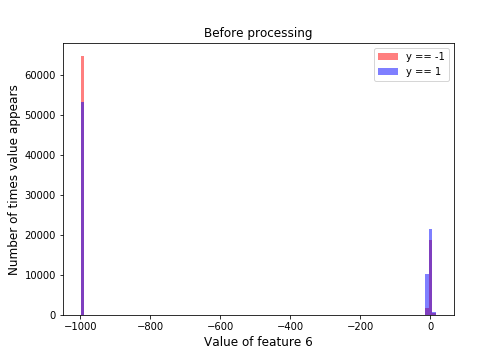
\includegraphics[width=\columnwidth]{graph-features/feature-06-raw.png}
  \caption{The feature 06 before processing}
	\label{fig:feature-06-raw}
\end{figure}

We noticed on figure \ref{fig:feature-06-raw} that the distribution is very strange and with this scale on the y-axis we can't really see exactly what's going on. But using this information and by going through the data there are features with many values set to exactly $-999$. Seems weird to have most of the values around 0 and a lot of them with exactly $-999$, we concluded that these values are in fact unknown.\\

Knowing that, we decided to normalize the data without taking into account the $-999$ values and then setting the $-999$ values to $0$. That way, they shouldn't have much impact on the decision, since $0 \times w$ will give 0, thus not contribute. Normalization is a good tool to avoid ill-conditioning and to balance the weight of each feature. You can see the plot at figure \ref{fig:feature-06-processed}.

\begin{figure}[h!]
	\centering
  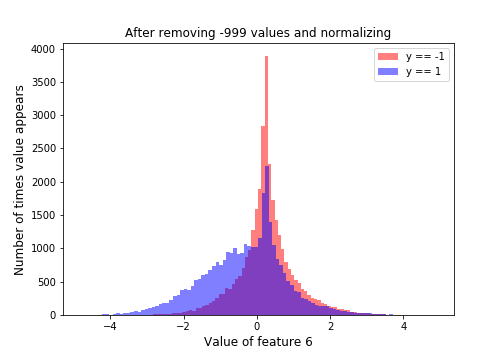
\includegraphics[width=\columnwidth]{graph-features/feature-06-processed.png}
  \caption{The feature 06 after processing, not displaying the $-999$ values}
	\label{fig:feature-06-processed}
\end{figure}

Another interesting thing we noticed, is that the 22nd feature is discrete. It only has 4 values: ${0,1,2,3}$, we thought that maybe this feature represents some category. Maybe they represent different particles. So we tried to train them differently. By normalizing the data as specified and training these 4 categories differently we managed to get to $78\%$ accuracy on training.

\section{Model choosing}
\label{sec:model-choosing}
The logistic regression seems to be inefficient on the data set since 

\section{Conclusion}
In conclusion, we started with a $66\%$ accuracy with no feature processing because of the unbalanced data. Then, we managed to up it to $78\%$ by analyzing data and processing the features, as explained in section \ref{sec:feature-engineering}. Then we got up to $82\%$ by adding feature expansion and valdiation, as described in section \ref{sec:model-choosing}. We use linear regression and based on our observations, we concluded that feature engineering is really the key to have a more successful classifier, the algorithm comes next. We unfortunately underestimated the importance of cleaning and processing the data. We lost a bit of time in the beginning, because we were trying to change the algorithm we run instead to have better results instead of changing the input.

\section{Further improvements}
To further improve the results we could try using other algorithms. We also noticed that some features have more unknown values to known values; some features look like uniform distribution or look like they don't give any information on the classification. We could try removing some of these features to reduce complexity. We could also dive into the actual physics behind the Higgs boson to have a better idea about what the best feature expansion looks like; we could try to add features that are redundant in the physics theory behind Higgs boson. There is always a lot more that can be done when working with machine learning, these are some clues we had while working on this project.

\begin{enumerate}
	\item{Copied 6 function we have to return from the labs}
	\item{Changed the functions we copied from the labs such that they always assume that vectors are represented in (N,1)}
	\item{Plotted distributions of features to gain insight}
	\item{Gradient descent on data to see what's going on}
	\item{Try to remove features based on the plots, the ones that look like they don't add anything}
	\item{Logistic regression, see if results make sense}
	\item{Try polynomial expansion to have better accuracy}
	\item{Try polynomial expansion with cross products to have better accuracy}
	\item{Realize that the weird distributions of many features with extreme variance are most likely due to the fact that -999 values are unknown values. Seems weird that many of the values are around zero, and many of them are exactly -999}
	\item{Normalize data without taking into account the -999 values, and set -999 values to 0. Such that they shouldn't affect the result as when 0 will be multiplied with the weight it'll be 0, i.e. not contribute.}
	\item{Re-plotted the distributions of the features after normalizing and removing the -999 values}
	\item{Notice that some plots look like uniform distribution or clearly don't give us insight on the result. => can remove them to have faster algorithm (NOT DONE YET)}
	\item{When plotting the distributions of features without unknown values we noticed something very strange: all of the distributions are continuous except one! It only has 4 values}
	\item{We thought that maybe this value is some sort of category, thus maybe we should treat them differently => we trained them separately, we separate them in 4 categories based on that feature and train them separately}
	\item{Trained the model that way with linear regression (no expansion), obtained much better results}
	\item{Tried logistic regression but results weren't as good}
	\item{Tried to add feature expansion, square and sqrt (without cross products)}
\end{enumerate}

\end{document}
